% !TEX TS-program = pdflatex
% !TEX encoding = UTF-8 Unicode

% This file is a template using the "beamer" package to create slides for a talk or presentation
% - Talk at a conference/colloquium.
% - Talk length is about 20min.
% - Style is ornate.

% MODIFIED by Jonathan Kew, 2008-07-06
% The header comments and encoding in this file were modified for inclusion with TeXworks.
% The content is otherwise unchanged from the original distributed with the beamer package.

\documentclass{beamer}


% Copyright 2004 by Till Tantau <tantau@users.sourceforge.net>.
%
% In principle, this file can be redistributed and/or modified under
% the terms of the GNU Public License, version 2.
%
% However, this file is supposed to be a template to be modified
% for your own needs. For this reason, if you use this file as a
% template and not specifically distribute it as part of a another
% package/program, I grant the extra permission to freely copy and
% modify this file as you see fit and even to delete this copyright
% notice. 


\mode<presentation>
{
  \usetheme{Warsaw}
  % or ...

  \setbeamercovered{transparent}
  % or whatever (possibly just delete it)
}


\usepackage[english]{babel}
% or whatever

\usepackage[utf8]{inputenc}
% or whatever

\usepackage{times}
\usepackage[T1]{fontenc}
% Or whatever. Note that the encoding and the font should match. If T1
% does not look nice, try deleting the line with the fontenc.


\title[] % (optional, use only with long paper titles)
{N-Body problem}

\subtitle
{A simulation study}

\author[S. Sultan, M. Boersma] % (optional, use only with lots of authors)
{S.~Sultan\inst{1} \and M.~Boersma\inst{1} }
% - Give the names in the same order as the appear in the paper.
% - Use the \inst{?} command only if the authors have different
%   affiliation.

\institute[Universities of Amsterdam] % (optional, but mostly needed)
{
  \inst{1}%
  Department of Computational Science\\
  University of Amsterdam
 }
% - Use the \inst command only if there are several affiliations.
% - Keep it simple, no one is interested in your street address.

\date[CFP 2003] % (optional, should be abbreviation of conference name)
{Introduction into Computational Sciences, 2014}
% - Either use conference name or its abbreviation.
% - Not really informative to the audience, more for people (including
%   yourself) who are reading the slides online

% This is only inserted into the PDF information catalog. Can be left
% out. 



% If you have a file called "university-logo-filename.xxx", where xxx
% is a graphic format that can be processed by latex or pdflatex,
% resp., then you can add a logo as follows:

% \pgfdeclareimage[height=0.5cm]{university-logo}{university-logo-filename}
% \logo{\pgfuseimage{university-logo}}



% Delete this, if you do not want the table of contents to pop up at
% the beginning of each subsection:
\AtBeginSubsection[]
{
  \begin{frame}<beamer>{Outline}
    \tableofcontents[currentsection,currentsubsection]
  \end{frame}
}


% If you wish to uncover everything in a step-wise fashion, uncomment
% the following command: 

%\beamerdefaultoverlayspecification{<+->}


\begin{document}

\begin{frame}
  \titlepage
\end{frame}

\begin{frame}{Outline}
  \tableofcontents
  % You might wish to add the option [pausesections]
\end{frame}


% Structuring a talk is a difficult task and the following structure
% may not be suitable. Here are some rules that apply for this
% solution: 

% - Exactly two or three sections (other than the summary).
% - At *most* three subsections per section.
% - Talk about 30s to 2min per frame. So there should be between about
%   15 and 30 frames, all told.

% - A conference audience is likely to know very little of what you
%   are going to talk about. So *simplify*!
% - In a 20min talk, getting the main ideas across is hard
%   enough. Leave out details, even if it means being less precise than
%   you think necessary.
% - If you omit details that are vital to the proof/implementation,
%   just say so once. Everybody will be happy with that.

\section{Motivation}

\begin{frame}{Motivation}
	\begin{itemize}
		\item
			Observational astronomy has limitations
		\item
			Computational models can describe evolution of systems that cannot be directly observed
		\item
			N-body deals with gravity, useful on scales where gravity dominates
	\end{itemize}
\end{frame}


\subsection{History}

\begin{frame}{Newton}
	\begin{itemize}
		\item
			Gravitation law \begin{equation} F = G \frac{m_1m_2}{r^2}\end{equation}
		\item 
        Net force on object (Newton's second law) \begin{equation} F = m \frac{dv}{dt} = ma \end{equation}
	\end{itemize}
\end{frame}


\subsection{2 Body problem}

\begin{frame}{2 Body problem}{A closed form solution}
  % - A title should summarize the slide in an understandable fashion
  %   for anyone how does not follow everything on the slide itself.

  \begin{itemize}
  \item
      Can be solved analytically, see \cite{frida2013}
  \item
      Pluto-Charon system, center of mass outside both bodies
  \item
  	What about $\geq$ 3-Bodies?
  \end{itemize}
\end{frame}

\begin{frame}{3 Body problem}
	We can not solve this analytical however we can calculate the acceleration, for each body and derive the change in position and speed from this.
  \begin{itemize}
    \item 
      Gravitation law on body $i$ : \begin{equation} F_i =G \sum_{k \neq i} \frac{m_im_k(r_k - r_i)}{|r_k - r_i|^3}\end{equation}
    \item 
      Acceleration $i$ : \begin{equation} a_i = G \sum_{k \neq i} \frac{m_k(r_k - r_i)}{|r_k - r_i|^3}\end{equation}
  \end{itemize}
  then, with $h$ as a time step, we can numerically derive the speed and position on $t+1$.
  
\end{frame}

\begin{frame}{Metrics}
Designing a metric to verify accuracy
 \begin{itemize}
	\item
		Conservation of momentum
	\item
		Conservation of energy
 \end{itemize}
\end{frame}

\begin{frame}{Conservation of momentum}
    \begin{itemize}
            \item
                For entire system: \begin{equation} \sum_{i=1}^{n} m_i \times \vec{v_i} \end{equation}
            \item
                Goes well almost always, even for bad integrators
    \end{itemize}
\end{frame}

\begin{frame}{Conservation of energy}
    \begin{itemize}
            \item
            Potential energy for system: \begin{equation} W = - 1/2 \sum_{i \ne j} G \frac{m_i m_j}{|\vec{r}_i-\vec{r}_j|}\end{equation}
            \item
            Kinetic energy for system: \begin{equation} K=1/2 \sum_{i=1}^{N} m_i |\vec{v}_i|^2 \end{equation}
            \item
                $K+W$ should be constant, according to law of conservation of energy
    \end{itemize}
\end{frame}
\section{Methods}

\begin{frame}{Naive approach}
  Fixed timestep $h$ and only an euler approximation
  \begin{itemize}
    \item
      speed: $V(t+1) = V(t) + A(t)*h$ 
    \item
      position: $X(t+1) = X(t) + V(t)*h$
    \item
      acceleration: \begin{equation} a_i = G \sum_{k \neq i} \frac{m_k(r_k - r_i)}{|r_k - r_i|^3}\end{equation}
  \end{itemize}

  hint: first order Taylor expansion
\end{frame}

\begin{frame}{Taylor expansion}
  One more term in the Taylor expansion, the "jerk"

  \begin{itemize}
    \item
        position: $X(t+1) = X(t) + V(t)*h + \frac{1}{2} A(t)*h^2 + \frac{1}{6} J(t) * h^3$
    \item
        speed: $B(t+1) = V(t) + A(t)*h + \frac{1}{2} J(t) * h^2$
    \item
        acceleration: $A(t+1) = A(t) + J(t) * h$
    \item
        jerk: \begin{equation} j_i = G \sum_{k \neq i} m_k \left( \frac{v_k - v_i}{|r_k - r_i|^3} - 3\frac{(r_k-r_i)\left((r_k - r_i)\cdot(v_k - v_i)\right)}{|r_k - r_i|^5} \right)
        \end{equation}
  \end{itemize}
\end{frame}

\begin{frame}{Leapfrog integration}
        Time reversible and better conservation of energy
    \begin{itemize}
        \item
            calculates position on times $t=0, t=1, t=2$ etc.
        \item
            calculates velocity on times $t=1/2, t=3/2, t=5/2$ etc.
    \end{itemize}
\end{frame}


\begin{frame}{Dynamic time scale}
  Can we improve it even further? Yes, we can!\\
  We can use dynamic time scales, and use the minimum implied timescale for $v(t),a(t)$. \\
  But how? With $r$ as the distance between two bodies, we can calculate the implied time scale:
  \begin{itemize}
    \item speed: $r/v= m/(m/s) = s$
    \item acceleration: $\sqrt{r/a} = \sqrt{m/(m/s^2)}  = \sqrt{s^2} = s$
  \end{itemize}
\end{frame}

\section{Our Results/Contribution}


\begin{frame}{The experiment}
  Run the following simulations:
  \begin{itemize}
    \item naive
    \item jerk
    \item leapfrog
  \end{itemize}
  with and without dynamic time scale.
\end{frame}

\begin{frame}{Results}
  Comparing the relative energy error:
  \begin{figure}
   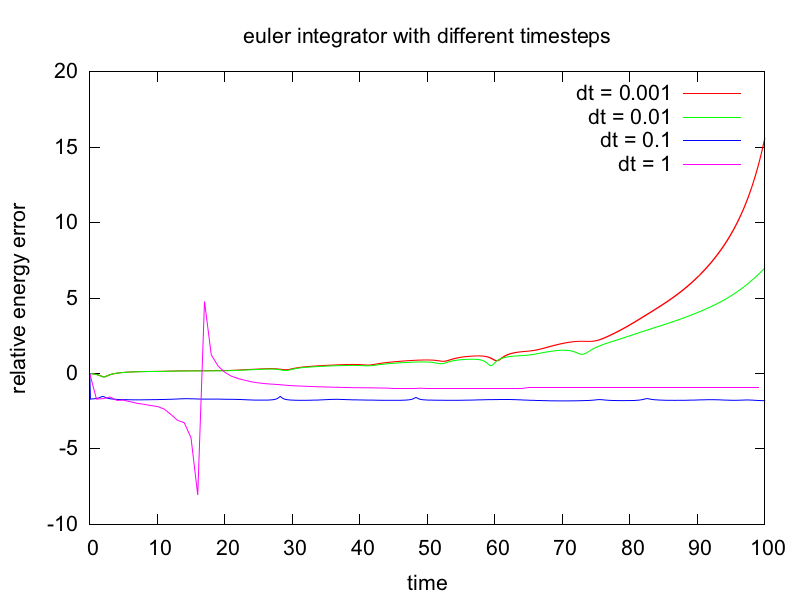
\includegraphics[width=0.6\paperwidth]{../results/euler_different_timesteps.png}
\end{figure}
\end{frame}

\begin{frame}{Results}
  Comparing the relative energy error:
  \begin{figure}
   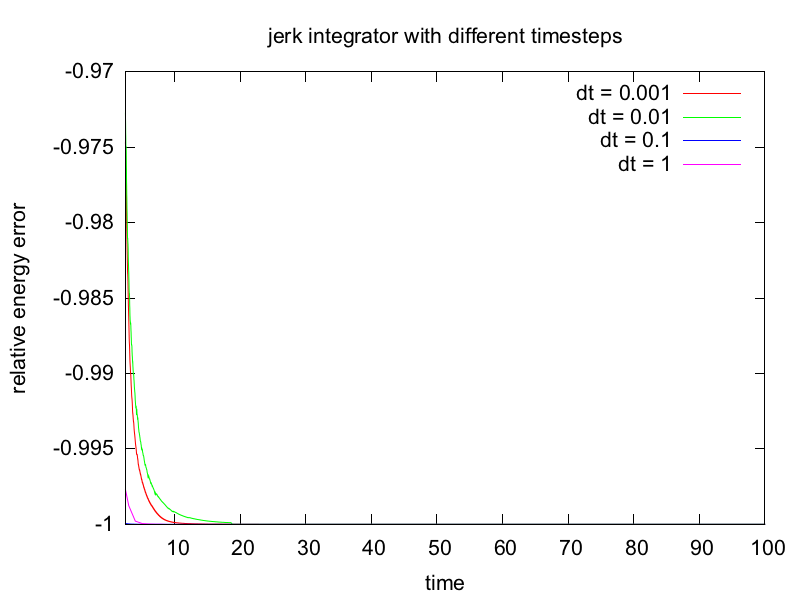
\includegraphics[width=0.6\paperwidth]{../results/jerk_different_timesteps_truncated.png}
\end{figure}
\end{frame}

\begin{frame}{Results}
  Comparing the relative energy error:
  \begin{figure}
   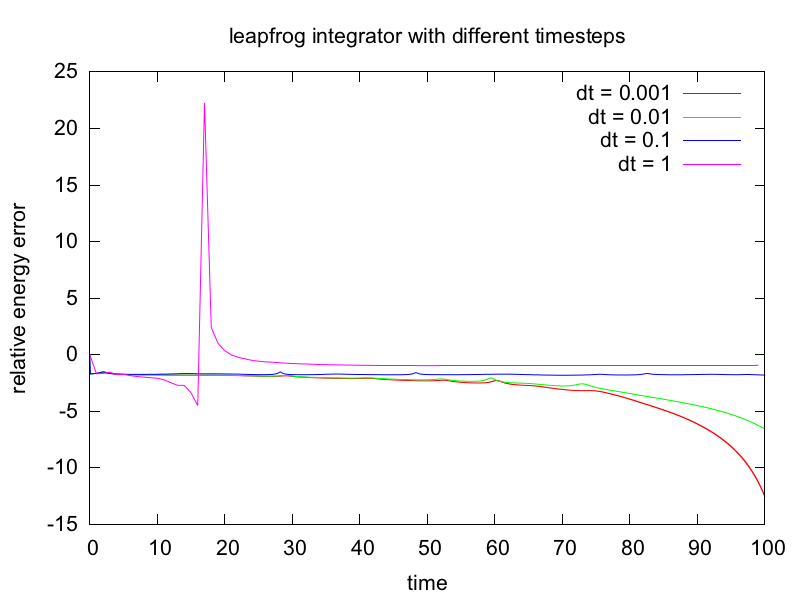
\includegraphics[width=0.6\paperwidth]{../results/leapfrog_different_timesteps.png}
\end{figure}
\end{frame}

\begin{frame}{Results}
  Comparing the relative energy error:
  \begin{figure}
   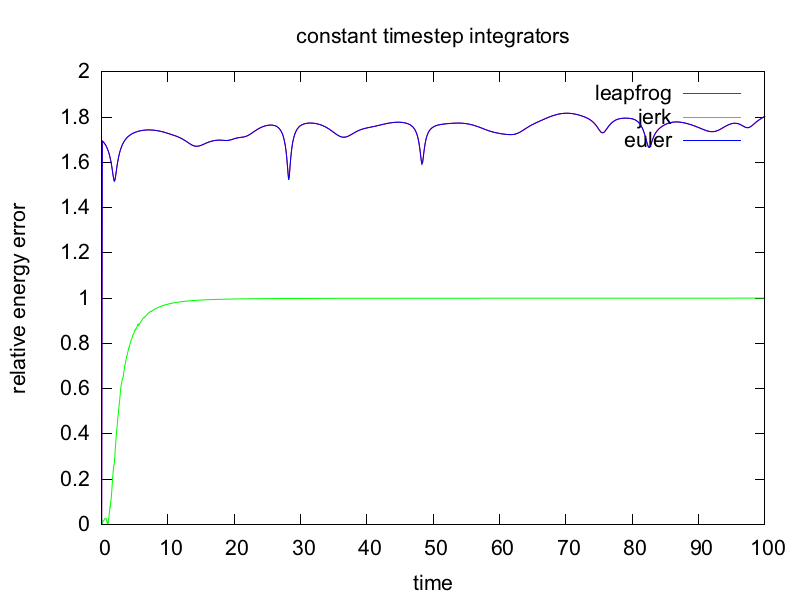
\includegraphics[width=0.6\paperwidth]{../results/constant_time.png}
\end{figure}
\end{frame}

\begin{frame}{Results}
  Comparing running time with different n:
  \begin{figure}
   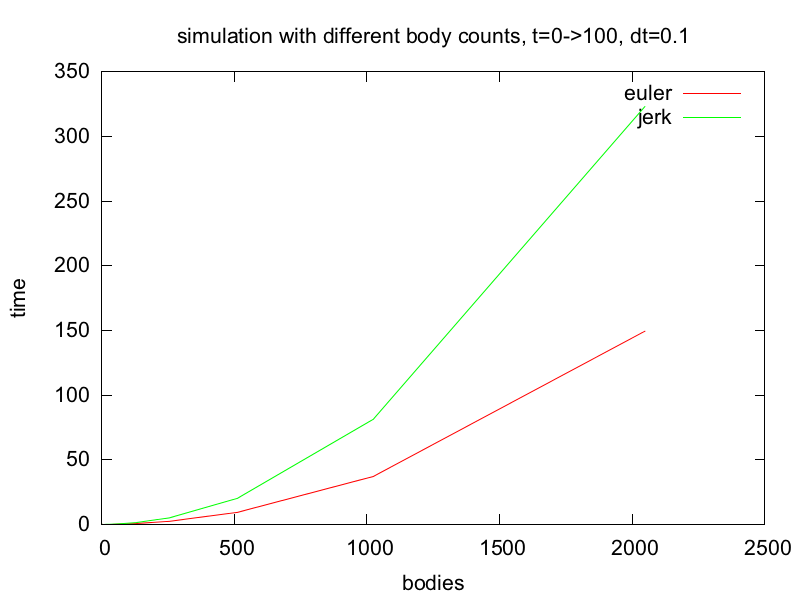
\includegraphics[width=0.6\paperwidth]{../results/time_bodies.png}
\end{figure}
\end{frame}

\section*{Summary}

\begin{frame}{Summary}

  % Keep the summary *very short*.
  \begin{itemize}
  \item
    Acceleration, speed and position directly from jerk doesn't give more accuracy.
\item
    Global dynamic timestep ends up with smallest possible timestep, so isn't really dynamic in that case.
  \end{itemize}
  
  % The following outlook is optional.
  \vskip0pt plus.5fill
  \begin{itemize}
  \item
    Future work
    \begin{itemize}
    \item
      Parallelize 
  \item
      Tree simulators vs. direct simulation
    \end{itemize}
  \end{itemize}
\end{frame}



% All of the following is optional and typically not needed. 
\appendix
\section<presentation>*{\appendixname}
\subsection<presentation>*{For Further Reading}

\begin{frame}[allowframebreaks]
  \frametitle<presentation>{For Further Reading}
    
  \begin{thebibliography}{10}
    
  \beamertemplatebookbibitems
  % Start with overview books.

 
    
  \beamertemplatearticlebibitems
  % Followed by interesting articles. Keep the list short. 

  \bibitem{frida2013}
    F.~Gleisner.
    \newblock Three solutions to the two-body problem.
    \newblock {\em Linaeus University BSc thesis}, 
    2013.
\bibitem{Dehnen}
    W.~Dehnen, J.~Read.
    N-body simulations of gravitational dynamics.
  \end{thebibliography}
\end{frame}

\end{document}


